\chapter{Обзор технологии обучения с подкреплением.} \label{ch1}

\section{Введение.} \label{ch1:intro}

Алгоритмы и методы глубокого обучения с подкреплением (Deep Reinforcement Learning, DRL) – это методы, которые мы используем для исследования вопросов дипломной работы. DRL – это подраздел машинного обучения, который лежит на пересечении Обучения с подкреплением (Reinforcement Learning) и глубокого обучения (Deep Learning). 

Прежде чем говорить о DRL, нужно кратко рассмотреть понятия, связанные с искусственным интеллектом и машинным обучением.

На \firef{fig:ch1-ML-and-AI-concepts} представлен обзор концепций, которые мы вводим в этой главе. 

Сначала мы рассмотрим искусственный интеллект, машинное обучение и его три категории. Затем мы углубимся в глубокое обучение. Наконец, мы рассмотрим основные алгоритмы DRL.
Таким образом, мы можем понять, почему и как DL и RL объединяются в DRL, который позволяет агентам взаимодействовать с более сложной средой и вести себя более разумно.

\begin{figure}[ht!] 
	\center
	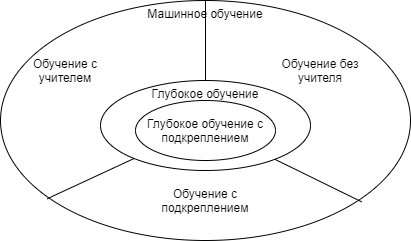
\includegraphics [scale=0.80] {my_folder/images/ch1/ML-and-AI-concepts.png}
	\caption{Граф, показывающий концепты МО и ИИ и их отношения.} 
	\label{fig:ch1-ML-and-AI-concepts}  
\end{figure}

\section{Искусственный Интеллект} \label{ch1:ai}

Искусственный интеллект \cite{Crevier93} (ИИ), как следует из названия, в отличие от естественного интеллекта человека и других животных, является искусственным. Именно такой тип интеллекта люди реализуют в машинах.
Конечной целью ИИ является создание таких автономных систем, которые способны учиться методом многочисленных проб и ошибок, чтобы найти оптимальное поведение для достижения максимально возможных целей в сложившемся окружении. \cite{RussellAndNorvig-AI-modern-approach}

С 21 века, благодаря нескольким прорывам, ИИ процветает в викторинах и настольных играх, превосходя уровень игры людей \cite{Watson} \cite{AlphaGo}. Наряду с увеличением вычислительной мощности, улучшения алгоритмов и доступности больших наборов данных, ИИ развивался революционными темпами. В ближайшем будущем, ИИ ещё сильнее повлияет на работу и повседневную жизнь человека.

\section{Машинное Обучение} \label{ch1:ml}

\subsection{Название первого подпараграфа первого параграфа первой главы для~демонстрации переноса слов в содержании} % ~ нужен, чтобы избавиться от висячего предлога (союза) в конце строки
